\documentclass[a4paper,10pt]{report}
\usepackage[francais]{babel}
\usepackage{ucs}
\usepackage[utf8x]{inputenc}
\usepackage[T1]{fontenc}
\usepackage[pdftex]{graphicx}
\usepackage{xcolor}
\usepackage{textcomp}
\usepackage[top=2cm, bottom=2cm, left=1.5cm, right=1.5cm]{geometry}
\usepackage{amsmath} 
\usepackage{amssymb}
\usepackage{mathrsfs}
\usepackage{graphicx}
\usepackage{pgfgantt}

\usepackage{listings}
\definecolor{colKeys}{rgb}{0,0,1}
\definecolor{colIdentifier}{rgb}{0,0,0}
\definecolor{-}{rgb}{0,0.5,1}
\definecolor{colString}{rgb}{0.6,0.1,0.1}
\definecolor{colBack}{rgb}{0.9,0.9,0.9}
\definecolor{colComments}{rgb}{0.5,0.5,0.5}
\definecolor{mygreen}{RGB}{28,172,0} % color values Red, Green, Blue
\definecolor{mylilas}{RGB}{170,55,241}


\lstdefinestyle{customc}
{
  belowcaptionskip=1\baselineskip,
  breaklines=true,
  frame=L,
  xleftmargin=\parindent,
  language=C,
  numbers=left,
  showstringspaces=false,
  basicstyle=\footnotesize\ttfamily,
  keywordstyle=\bfseries\color{green!40!black},
  commentstyle=\itshape\color{purple!40!black},
  identifierstyle=\color{blue},
  stringstyle=\color{orange},
  tabsize=4,
}

\lstdefinestyle{customasm}
{
  belowcaptionskip=1\baselineskip,
  frame=L,
  xleftmargin=\parindent,
  language=[x86masm]Assembler,
  basicstyle=\footnotesize\ttfamily,
  commentstyle=\itshape\color{purple!40!black},
}

\lstset{language=Matlab,%
    %basicstyle=\color{red},
    breaklines=true,%
    morekeywords={matlab2tikz},
    keywordstyle=\color{blue},%
    morekeywords=[2]{1}, keywordstyle=[2]{\color{black}},
    identifierstyle=\color{black},%
    stringstyle=\color{mylilas},
    commentstyle=\color{mygreen},%
    showstringspaces=false,%without this there will be a symbol in the places where there is a space
    numbers=left,%
    numberstyle={\tiny \color{black}},% size of the numbers
    numbersep=9pt, % this defines how far the numbers are from the text
    emph=[1]{for,end,break},emphstyle=[1]\color{red}, %some words to emphasise
    %emph=[2]{word1,word2}, emphstyle=[2]{style},    
}

\lstset{escapechar=@,style=customc}

% Title Page
\title{Rapport MT44\\\huge{TP2}}
\author{Nicolas Fleurot\\Tony Duong}

\begin{document}
\maketitle

\tableofcontents

\chapter*{Introduction}
\addcontentsline{toc}{chapter}{Introduction}

Les courbes de Bézier ont été inventées en 1962 par Pierre Bézier, ingénieur chez Renault. Les courbes de Bézier sont des courbes polynomiales paramétriques qui ont été utilisées à l’origine pour concevoir des pièces d’automobile à l’aide d’ordinateurs. Le dessin vectoriel, la CAO et toutes les activités de design industriel à partir de “dessin” sur ordinateur s’appuient sur la construction géométrique des courbes de Béziers. Aujourd’hui, elles ont de nombreuses applications dans la synthèse d’images et le rendu de polices de caractères. \\

Après les courbes de Bézier, nous nous intéressons aux courbes splines. Les B-splines sont une généralisation des courbes de Bézier et offrent beaucoup plus de souplesse en terme de manipulation et de réalisation. Elles permettent également de réaliser des courbes que les Bézier ne peuvent pas. \\

Dans une première partie, nous nous intéresserons aux courbes de Bézier et à leur construction. Pour cela, nous étudierons l’algorithme de Casteljau et l’implémenterons afin de pouvoir créer des courbes à partir de points de contrôle.\\

Dans une seconde partie, après les courbes de Bézier, nous passerons aux courbes splines et étudierons leur construction. En s’inspirant de l’algorithme de de Boor-Cox, nous créerons une fonction permettant de construire et d’afficher les B-splines de degré variable pour un vecteur noeud donné.\\

Enfin, on illustrera l’utilisation des courbes de Bézier en dessinant la lettre alpha en utilisant une Bézier de degré trois (donc avec quatre points de contrôle $P0$, $P1$, $P2$, $P3$). On dilatera et rotatera cette lettre en modifiant les positions des points de contrôle.

\chapter*{Partie 1 : Algorithme de de Casteljau}
\addcontentsline{toc}{chapter}{Partie 1 : Algorithme de de Casteljau}

\section*{Question 1a et 1b}
\addcontentsline{toc}{section}{Question 1a}

\subsection*{Rappel}
\addcontentsline{toc}{subsection}{Rappel}

On rappelle qu'il s'agit de l'algorithme classiquement utilisé pour la création des courbes de Bézier.

Il a été fourni et étudié en cours. Nous en rappelons la structure ci-dessous ; 
on définit la fonction $casteljau(P_{0} , ..., P_{n}, t \rightarrow P_{n}^{n}(t))$ comme suit :

\textbf{entrée :}

\begin{list}{}{}
\item $n+1$ points $P_{0}$, ..., $P_{n}$ de $\varepsilon$ par leurs coordonnées dans le repère ($O, \vec{i}, \vec{j}, \vec{k}$).
\item $t$ réel élément de $[0, 1]$

\end{list}

\textbf{sortie :} Coordonnées de $P^{n}_{n}(t)$\\

\textbf{Corps d'algorithme}

Début
\begin{list}{}{}
\item Initialisation\\Pour tout $i$ : $P_{i}^{0} \leftarrow P_{i}$
\item \textbf{pour} r = 0 jusqu'à $n-1$ \textbf{faire}
\item \begin{list}{}{}
\item \textbf{pour} i = r jusqu'à $n-1$ \textbf{faire}
\item \begin{list}{}{}
\item $P^{r+1}_{i+1}(t) \leftarrow (1 - t)P^{r}_{i}(t) + tP^{r}_{i+1}(t)$
\end{list}
\item \textbf{fin pour}
\end{list}
\item \textbf{fin pour}
\item Sortie de $P^{n}_{n}(t)$
\end{list}

\textbf{Fin du corps}

\subsection*{Théorie}
\addcontentsline{toc}{subsection}{Théorie}

Pour construire une courbe de Bézier, on aura besoin d’un ensemble de points de contrôles $P_{0}, P_{1}, P_{2}, …, P_{n}$ et d’un paramètre $t$ appartenant à $[0,1]$. Grâce à ces points de contrôle d’origine, nous pourrons construire des points de contrôle “fils” qui à leur tour, permettrons de construire encore d’autres points de contrôle. 

Dans le cas général, la relation liant les $P$ de rang $r$ et les $P $de rang $r-1$ est 

\begin{equation}
    P^{r}_{i+1}(t) = (1-t)P^{r-1}_{i}(t)+tP^{r-1}_{i+1}(t), r \in [1, n], i \in [r, n]
\end{equation}

Après cette explication théorique, nous implémentons l’algorithme de Casteljau afin de générer tous ces points Pn,n et ainsi afficher la courbe générée.
    
\newpage
\subsection*{Source}
\addcontentsline{toc}{subsection}{Source}

\begin{center}
	\lstinputlisting[caption=, language=Matlab]{CastelJau.m}
\end{center}

\subsection*{Test}
\addcontentsline{toc}{subsection}{Test}

\begin{center}
%	\lstinputlisting[caption=Test evaluation1, language=Matlab]{testevaluation1.m}
\end{center}

\newpage
\section*{Question 1c}
\addcontentsline{toc}{section}{Question 1b}

\subsection*{Rappel}
\addcontentsline{toc}{subsection}{Rappel}

Proposer une visualisation des points de contrôle $P_{0} , ..., P_{n}$ et de la naissance des points $P_{n}^{n}(t)$. 

\subsection*{Théorie}
\addcontentsline{toc}{subsection}{Théorie}

\begin{figure}[h]
	\begin{center}
		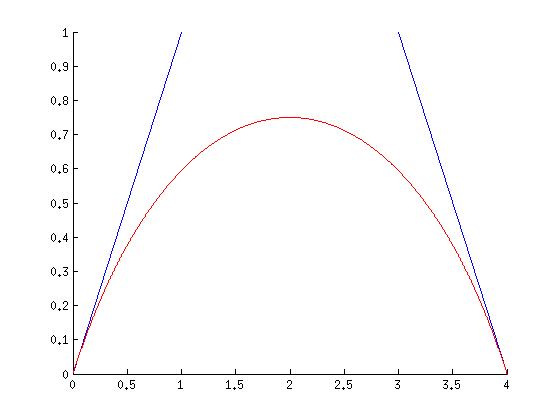
\includegraphics[scale=0.8]{visualiseCastle}
		\caption{Courbe de bézier de 4 points}
	\end{center}
\end{figure}


\subsection*{Source}
\addcontentsline{toc}{subsection}{Source}

\begin{center}
	\lstinputlisting[caption=VisualiseCastelJau.m, language=Matlab]{VisualiseCastelJau.m}
\end{center}

\subsection*{Test}
\addcontentsline{toc}{subsection}{Test}

\newpage
\section*{Question 1d}
\addcontentsline{toc}{section}{Question 1b}

\subsection*{Rappel}
\addcontentsline{toc}{subsection}{Rappel}

Que proposeriez-vous comme logiciel de démonstration, destiné à faire saisir à un étudiant qui découvre les Bézier, la manière dont se construisent les points relatifs à chaque valeur de t ?
\subsection*{Théorie}
\addcontentsline{toc}{subsection}{Théorie}

\begin{figure}[h]
	\begin{center}
		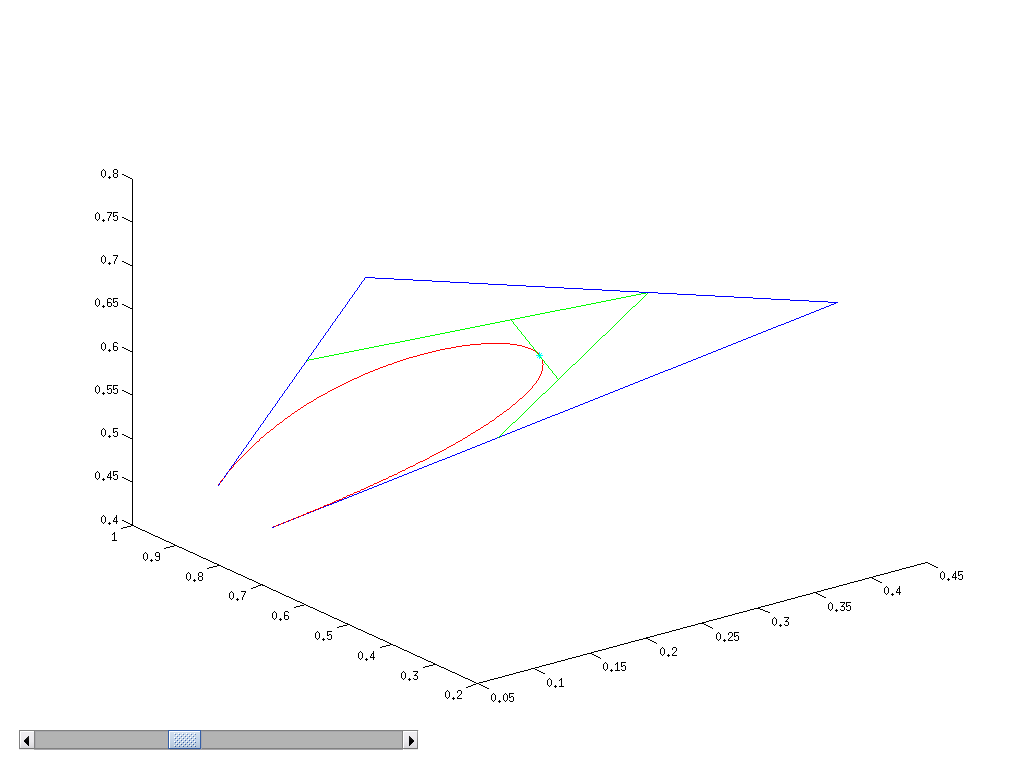
\includegraphics[scale=0.6]{guiCastle}
		\caption{Courbe de bézier de 4 points}
	\end{center}
\end{figure}


\subsection*{Source}
\addcontentsline{toc}{subsection}{Source}

\begin{center}
	\lstinputlisting[caption=, language=Matlab, mathescape]{GUICastleJauTex.m}
\end{center}

\subsection*{Test}
\addcontentsline{toc}{subsection}{Test}

\chapter*{Partie 2 : Étude des $B^{i}_{k}$}
\addcontentsline{toc}{chapter}{Partie 1 : Algorithme de de Casteljau}

\subsection*{Rappel}
\addcontentsline{toc}{subsection}{Rappel}

Écrire une fonction génère $B_{i,k}$ qui, à partir d’un vecteur noeud $t$ (constitué de valeurs distinctes ou confondues en nombre adéquat pour demeurer cohérent avec le reste des données) et de l’entier $k$ inférieur ou égal à 4, fournit la définition de la fonction $B_{i,k}$, pour tout indice $i$ convenable.\\

Adjoindre à la fonction antérieure un champ complémentaire trace qui, lorsqu’il sera égal à 1, fournira la représentation graphique des $B_{i,k}$ sur un intervalle convenable.


\subsection*{Théorie}
\addcontentsline{toc}{subsection}{Théorie}

Considérons une suite dans $\mathbb{R}$ $t_0 \leqslant t_1 \leqslant … \leqslant t_m$. $(t_0, t_1, …, t_m)$ est appelé le vecteur noeud. 

On définit par récurrence les fonctions B-splines $B_{i,k}$ pour $i = 0, … , m-k-1$ par les relations suivantes :

\begin{equation}
	\begin{array}{ll}
	B_{i,0} = \left\{
                \begin{array}{ll}
                  1 $ si $x \in [t_{i}, t_{i+1}[\\
                  0 $ sinon$
                \end{array}
              \right.\\              
    B_{i,k} = \omega_{i, k}(x)B_{i,k-1}(x) + (1 - \omega_{i+1, k}(x)B_{i+1,k-1}(x)$ si $ k \geqslant 1
    \end{array}
\end{equation}

Chaque fonction $B_{i,k}$ est construite par morceaux. En effet, les fonctions $B_{i,k}(x)$ auront pour chaque intervalle $[t_i,t_{i+1}]$ une fonction différente.



\subsection*{Source}
\addcontentsline{toc}{subsection}{Source}

\begin{center}
	\lstinputlisting[caption=genere\_bik, language=Matlab, mathescape]{genere_bikTex.m}
\end{center}

\subsection*{Test}
\addcontentsline{toc}{subsection}{Test}

\begin{figure}[h]
	\begin{center}
		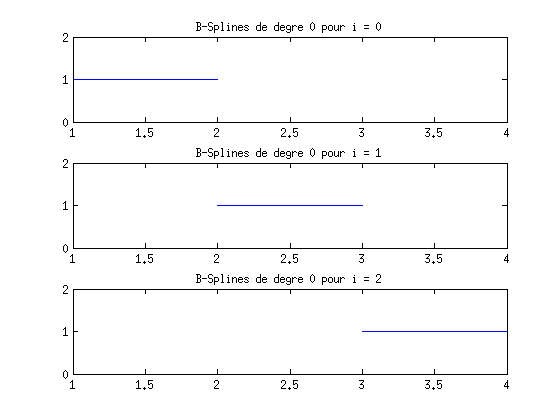
\includegraphics[scale=0.6]{bik}
		\caption{Courbe B-Spline de degrée 0 pour les points $[1, 2, 3, 4]$}
	\end{center}
\end{figure}

\begin{figure}[h]
	\begin{center}
		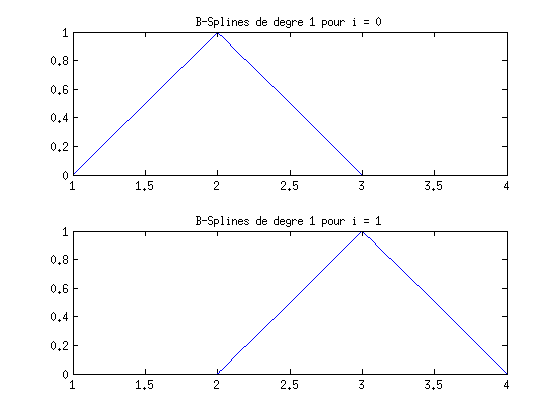
\includegraphics[scale=0.6]{bik2}
		\caption{Courbe B-Spline de degrée 1 pour les points $[1, 2, 3, 4]$}
	\end{center}
\end{figure}

\begin{figure}[h]
	\begin{center}
		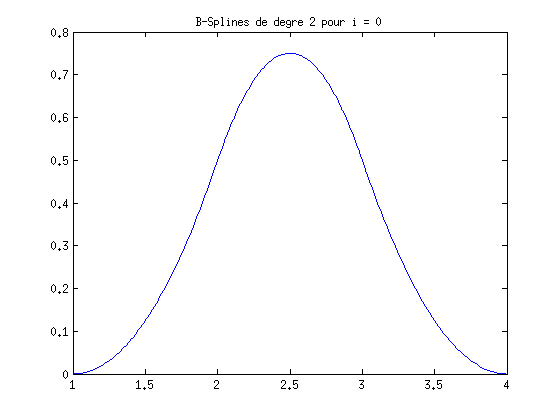
\includegraphics[scale=0.6]{bik3}
		\caption{Courbe B-Spline de degrée 2 pour les points $[1, 2, 3, 4]$}
	\end{center}
\end{figure}

\chapter*{Partie 3 : Exemple d’utilisation en imprimerie}
\addcontentsline{toc}{chapter}{Partie 3 : Exemple d’utilisation en imprimerie}

\section*{Création de la lettre alpha}
\addcontentsline{toc}{subsection}{Création de la lettre alpha}

\subsection*{Rappel}
\addcontentsline{toc}{subsection}{Rappel}

Écrire une fonction \textbf{creation alpha} permettant de dessiner la lettre alpha en utilisant une Bézier de degré trois, et donc quatre points de contrôle, $P_0$, $P_1$, $P_2$ , $P_3$ qui en constituent les champs d’entrée.

\subsection*{Source}
\addcontentsline{toc}{subsection}{Source}

\begin{center}
	\lstinputlisting[caption=genere\_bik, language=Matlab]{creation_alpha.m}
\end{center}

\newpage
\subsection*{Test}
\addcontentsline{toc}{subsection}{Test}

\begin{figure}[h]
	\begin{center}
		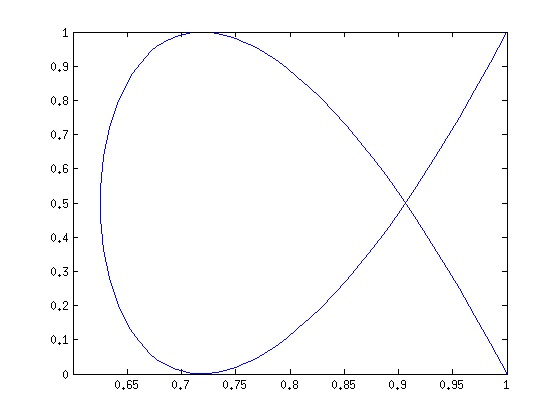
\includegraphics[scale=0.6]{alpha}
		\caption{Lettre alpha}
	\end{center}
\end{figure}


\section*{Dilatation et rotation d'une lettre}
\addcontentsline{toc}{subsection}{Test}

\subsection*{Rappel}
\addcontentsline{toc}{subsection}{Rappel}

\begin{list}{$\bullet$}{}
\item Écrire une fonction qui permet de tracer la lettre alpha ”dilatée”, dans une homothétie de centre $I$ de rapport $k \neq 0$. Choisir un centre $I$ satisfaisant. Comment mettre en place la lettre dilatée dans un texte?

\item Mêmes questions adaptées dans le cas de la rotée de la lettre alpha.

\end{list}

\subsection*{Théorie}
\addcontentsline{toc}{subsection}{Théorie}

Pour dilater et roter toute la lettre alpha, il suffit de modifier la position des points de contrôles d’origine par l’homothétie ou la rotation et de recréer la lettre après ces déplacements.

La position d’un point $S’$ obtenue par homothétie de rapport $k$ et de centre $O$ à partir d’un point $S$ est 

\begin{equation}
	S' = (S - 0) * k
\end{equation}

La position d’un point $S’$ obtenue par rotation d’angle $k$ et de centre $O$ à partir d’un point $S$ est 

\begin{equation}
	\begin{array}{ll}
		S'(x) = \cos(k) * (S(x)-O(x)) - \sin(k) * (S(x) - O(x))+O(x)\\
		S'(y) = \sin(k) * (S(y)-O(y)) - \cos(k) * (S(y) - O(y))+O(x)
	\end{array}
\end{equation}


\subsection*{Source}
\addcontentsline{toc}{subsection}{Source}

\begin{center}
	\lstinputlisting[caption=Dilater\_alpha, language=Matlab]{dilatation_alpha.m}
\end{center}

\begin{center}
	\lstinputlisting[caption=Rotation\_alpha, language=Matlab]{rotation_alpha.m}
\end{center}

\subsection*{Test}
\addcontentsline{toc}{subsection}{Test}

\begin{figure}[h]
	\begin{center}
		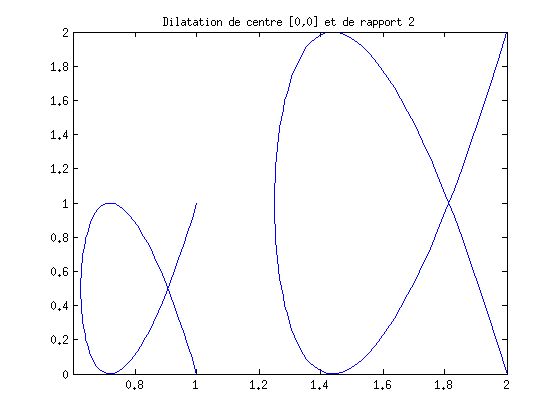
\includegraphics[scale=0.7]{dilate}
		\caption{Lettre alpha dilater de centre $(0, 0)$ de rapport 2}
	\end{center}
\end{figure}

\begin{figure}[h]
	\begin{center}
		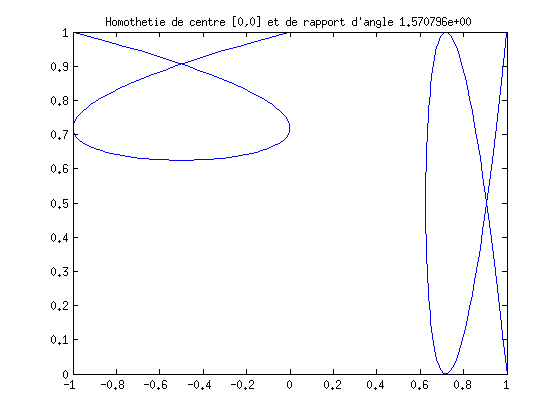
\includegraphics[scale=0.7]{rotate}
		\caption{Lettre alpha roter de centre $(0, 0)$ d'angle $\frac{\pi}{2}$}
	\end{center}
\end{figure}

\chapter*{Conclusion}
\addcontentsline{toc}{chapter}{Conclusion}

La problématique de ce chapitre a été de pouvoir trouver une fonction polynôme qui passerait par un nombre fini de points d’un certain support (obtenus par mesures par exemples). Il existe plusieurs méthodes pour arriver à ce but.
\newline
\newline
Dans ce TP, nous avons utilisé la méthode de Newton et avons produit deux algorithmes permettant d’évaluer la fonction en un point quelconque t. La fonction supposait que l’on connaissait à l’avance les coefficients de l’écriture de Newton.
\newline
\newline
Le premier algorithme produit est classique : il consiste à calculer les polynômes $(x-c)$ où $c$ est un point du support et à multiplier ceux-ci par leurs coefficients respectifs. Néanmoins, cette méthode génère des répétitions et n’est donc pas optimal en terme de temps d’éxécution.
\newline
\newline 
La seconde méthode tiré du Schéma de Horner n’a pas ce défaut. En effet, étant donné que les facteurs $(x-c)$ sont répétés dans l’écriture, il était préférable d’ajouter les facteurs déjà calculés aux les termes suivants de la somme.
\newline
\newline
La mesure du temps d’exécution confirme notre affirmation.
\newline
\newline
Par la suite, nous nous sommes intéressés par l’écriture de la fonction interpôlante en générant la table des différences divisées (qui contient les coefficients de Newton) et en écrivant cette écriture sous forme de chaîne de caractères. Nous devions ensuite interpôler la fonction exponentielle. 
\newline
\newline
Mais la question la plus importante concerne l’erreur commise en faisant cette approximation et le choix des points de support. L’erreur aux points de support est bien sûr nulle mais qu’en est-il des autres points ? 
\newline
\newline
Nous avons observé que l’erreur (pour les deux fonctions d'interpolation) grandissait au fur et à mesure qu’on s’éloignait des points de support. En ce qui concerne le choix entre les deux supports(équi-distants ou Tchebyschev), nous ne voyons pas immédiatement la différence sur l'exemple de ce TP, mais utiliser les points de Tchebyschev permet d'atténuer le phénomène de Runge qui rend "instable" la courbe d'interpolation : plus on ajoute de points sur le support, plus la courbe sera "instable" au bord. En concentrant les points de supports aux extrémités de l'intervalle, ce phénomène est affaibli et on obtient une meilleure approximation globale. 


\end{document}